% !TEX root = main.tex

\section{Experiments}
\label{sec:exp}

In this section, we present our experimental study.
We use DBpedia2014~\cite{dbpedia} and Probase~\cite{wu2012probase} as our knowledge repository.
We use entity pair as well as their attributes in DBpedia to learn the conceptual patterns.
We Probase for conceptualization. We carry out all the experiments on a PC with Intel i7 cpu @2.5Ghz and 16G memory.
All the programs implemented in Python 2.7.

\paragraph*{Evaluation Metrics}
Given two entities, our system produce the most plausible top-K attributes between the 2 entities.
We want to evaluate how accurate the result is. Hence we use $nDCG@K$ and $Precision@K$ as our evaluation metric.
We report the $MAP@K$ (Mean Average Precision at K) as well.
{\bf  In the case of finding plausible concept pairs for a given attribute, we further use $ ERR@10$~\cite{chapelle2009expected} to evaluate the expected reciprocal rank analogizing the process of limiting $C-C$ space to $topK^2$ to the act of a user stopping his search at the K-th concept.
}


\subsection{Exp1: Effectiveness of ERF}
In this subsection, we evaluate the effectiveness of our ERF system.
For comparison, we use the ...as baseline.....
We report all the precision metrics in Table~\ref{tab:ndcg}.

\begin{table}[htbp]
  \centering
  \caption{Evaluation Result}
    \begin{tabular}{rr}
    \toprule
    mesure & value \\
    \midrule
    nDCG@3 & 0.945 \\
    nDCG@5 & 0.941 \\
    precision@3 & 0.88 \\
    precision@5 & 0.76 \\
    MAP@3 & 0.902 \\
    MAP@5 & 0.907 \\

    \bottomrule
    \end{tabular}%
  \label{tab:ndcg}%
\end{table}%


We use the direct retrieval as a baseline.
We randomly select 50 Wikipedia article, and take only the hyper-linked entities abstract part as evaluation.
We consider the linked entities as the $e_2$ of the relation explanation input and source entity as $e_1$.
Compared with baseline, i.e. DBpedia original.
Since we assume 0 if the entity has no relation can be retrieved from database and otherwise 1, the average $Precision@1$ results here can also be viewed as \ac{recall} of the knowledge base.
DBpedia provides only one relation for a covered entity pair, therefore we use $Precision@1$ to compare the results.
Our ERF method improves the average $Precision@1$ by 15.77\%.
The result is reported in Table~\ref{tab:precision_compare}

\begin{table}[htbp]
  \centering
  \caption{Precision@1 Compared With Baseline}
    \begin{tabular}{rrr}
    \toprule
         & P@1  & \%Improv. \\
    \midrule
    Dbpedia direct & 0.64 & -- \\
    ERF  & 0.83 & 15.77 \\
    \bottomrule
    \end{tabular}%
  \label{tab:precision_compare}%
\end{table}%






\subsection{Exp 2: Head-aware Conceptulization}
We show that head-aware conceptualization first significantly reduce the computation cost. 
In Table~\ref{tab:nhc}, we report the changes of the $Probase$ concept space when applied our conceptualize method, where we have 33197 head concepts after doing the head modifier detection, while 2 million concepts before.

The increase of the average occurrence indicates the confidence of the $e$\isa$c$ pair is increased.
The increase of the average children per concept makes entities less unique, which will help avoid entity with same head concept share no long concept.

\begin{table}[htbp]
  \centering
  \caption{Necessity of Head Conceptualization}
    \begin{tabular}{rrrr}
    \toprule
          & Before & After & Changed\% \\
    \midrule
    concept number & 2127953 & 33197 & -98.44 \\
    average occurrence & 1.75  & 2.71  & 54.85714 \\
    children per concept & 7.53  & 184.3 & 2347.543 \\
    parents per entity & 2.33  & 1.55  & -33.4764 \\
    \bottomrule
    \end{tabular}%
  \label{tab:nhc}%
\end{table}%


... We give the distribution of head give an entity... We report the Pearson correlation between....

We further give case studies in Table.~\ref{tab:rerank} with the comparison to the direct estimation of $P(c|e)$ using Probase. We can see that
%
%\begin{table*}[htbp!]
%  \centering
%  \caption{Rerank comparation}
%    \begin{tabular}{llrrlrr}
%    \toprule
%    \multicolumn{1}{c}{} & \multicolumn{3}{c}{aggregated} & \multicolumn{3}{c}{original head concepts} \\
%    \midrule
%    \multicolumn{1}{c}{Entity} & agg head & agg count & agg prob & org head & org count & org prob \\
%    \midrule
%    \multicolumn{1}{c}{\multirow{10}[0]{*}{shanghai}} & city  & 1311  & 0.829222 & city  & 644   & 0.407337 \\
%    \multicolumn{1}{c}{} & region & 46    & 0.029096 & region & 27    & 0.017078 \\
%    \multicolumn{1}{c}{} & area  & 42    & 0.026565 & metropolis & 23    & 0.014548 \\
%    \multicolumn{1}{c}{} & metropolis & 26    & 0.016445 & megacities & 15    & 0.009488 \\
%    \multicolumn{1}{c}{} & port  & 20    & 0.01265 & market & 15    & 0.009488 \\
%    \multicolumn{1}{c}{} & market & 19    & 0.012018 & location & 15    & 0.009488 \\
%    \multicolumn{1}{c}{} & centre & 18    & 0.011385 & port  & 9     & 0.005693 \\
%    \multicolumn{1}{c}{} & location & 17    & 0.010753 & locality & 6     & 0.003795 \\
%    \multicolumn{1}{c}{} & megacities & 15    & 0.009488 & locale & 5     & 0.003163 \\
%    \multicolumn{1}{c}{} & center & 11    & 0.006958 & seaport & 4     & 0.00253 \\
%          &       &       &       &       &       &  \\
%    \multicolumn{1}{c}{\multirow{10}[0]{*}{bill gates}} & leader & 46    & 0.140244 & billionaire & 37    & 0.112805 \\
%    \multicolumn{1}{c}{} & billionaire & 44    & 0.134146 & entrepreneur & 28    & 0.085366 \\
%    \multicolumn{1}{c}{} & entrepreneur & 41    & 0.125 & philanthropist & 23    & 0.070122 \\
%    \multicolumn{1}{c}{} & philanthropist & 30    & 0.091463 & celebrity & 15    & 0.045732 \\
%    \multicolumn{1}{c}{} & celebrity & 20    & 0.060976 & leader & 9     & 0.027439 \\
%    \multicolumn{1}{c}{} & person & 16    & 0.04878 & innovator & 6     & 0.018293 \\
%    \multicolumn{1}{c}{} & figure & 11    & 0.033537 & personality & 5     & 0.015244 \\
%    \multicolumn{1}{c}{} & innovator & 8     & 0.02439 & expert & 5     & 0.015244 \\
%    \multicolumn{1}{c}{} & luminary & 8     & 0.02439 & folks & 4     & 0.012195 \\
%    \multicolumn{1}{c}{} & individual & 7     & 0.021341 & icon  & 4     & 0.012195 \\
%          &       &       &       &       &       &  \\
%    \multicolumn{1}{c}{\multirow{10}[0]{*}{samsung}} & company & 1030  & 0.376875 & company & 816   & 0.298573 \\
%    \multicolumn{1}{c}{} & brand & 829   & 0.30333 & brand & 561   & 0.205269 \\
%    \multicolumn{1}{c}{} & manufacturer & 238   & 0.087084 & client & 42    & 0.015368 \\
%    \multicolumn{1}{c}{} & maker & 112   & 0.040981 & firm  & 39    & 0.01427 \\
%    \multicolumn{1}{c}{} & player & 60    & 0.021954 & rival & 38    & 0.013904 \\
%    \multicolumn{1}{c}{} & phone & 60    & 0.021954 & player & 33    & 0.012075 \\
%    \multicolumn{1}{c}{} & giant & 51    & 0.018661 & phone & 30    & 0.010977 \\
%    \multicolumn{1}{c}{} & firm  & 49    & 0.017929 & conglomerate & 19    & 0.006952 \\
%    \multicolumn{1}{c}{} & name  & 49    & 0.017929 & corporation & 19    & 0.006952 \\
%    \multicolumn{1}{c}{} & conglomerate & 42    & 0.015368 & partner & 12    & 0.004391 \\
%          &       &       &       &       &       &  \\
%    \multicolumn{1}{c}{\multirow{10}[0]{*}{mona lisa}} & painting & 56    & 0.4   & painting & 33    & 0.235714 \\
%    \multicolumn{1}{c}{} & masterpiece & 21    & 0.15  & masterpiece & 16    & 0.114286 \\
%    \multicolumn{1}{c}{} & work  & 20    & 0.142857 & work  & 10    & 0.071429 \\
%    \multicolumn{1}{c}{} & film  & 6     & 0.042857 & film  & 5     & 0.035714 \\
%    \multicolumn{1}{c}{} & image & 5     & 0.035714 & image & 3     & 0.021429 \\
%    \multicolumn{1}{c}{} & artwork & 4     & 0.028571 & picture & 3     & 0.021429 \\
%    \multicolumn{1}{c}{} & portrait & 4     & 0.028571 & treasure & 2     & 0.014286 \\
%    \multicolumn{1}{c}{} & piece & 4     & 0.028571 & song  & 2     & 0.014286 \\
%    \multicolumn{1}{c}{} & picture & 3     & 0.021429 & icon  & 2     & 0.014286 \\
%    \multicolumn{1}{c}{} & figure & 3     & 0.021429 & artwork & 1     & 0.007143 \\
%    \bottomrule
%
%    \end{tabular}%
%  \label{tab:rerank}%
%\end{table*}%



%\subsection{Find alias}

%\subsubsection{compare}
%
%In this section we compare $ P(<c_1,c_2 >|a )$ with $ P(c_1|a) \times P(c_2|a)$ to show that

\subsection{Exp 3: Joint Conceptulization}
Now, we evaluate the effectiveness joint conceptualization, which is implemented by the introduction of $\alpha(c_1,c_2)$ in Eq.~\ref{eq:target_expand2_jr}. We compare to the baseline method in Eq~\ref{eq:naive}.
We present Table~\ref{tab:expjc} to show many cases where $\alpha$ help identify the true concept pair (ranked as the first).
Due to space limit, we place the entity with multiple meaning at $e_1$ and present result of $c_1$ only.
\begin{table}[htbp]
  \centering
  \caption{Joint Conceptualization with and without $\alpha$}
    \begin{tabular}{rrrr}
    \toprule
    $e_1$                               & $e_2$                               & $c_1 $  without $\alpha$       & $c_1$  with $\alpha$ \\
    \midrule
    columbia                            & barack obama                        & country                    & \textbf{school }\\
    apple                               & steve jobs                          & fruit                & \textbf{company} \\
   da vinci code           & ron howard                       & book                     & \textbf{film} \\
    spa                                 & belgium                             & facility                  & \textbf{place} \\
    \bottomrule
    \end{tabular}%
  \label{tab:expjc}%
\end{table}%



%
%{\bf Since there are many entities belongs to the same concept and we only consider topK $(c_1,c_2)$ pairs that has high typicality $P( (c_1,c_2) |a)$, so that the weird $(c_1,c_2)$ patterns as manifest in Example.~\ref{exa:sd} can be easily filtered.}
%
%\begin{figure}[!htb]
%\centering 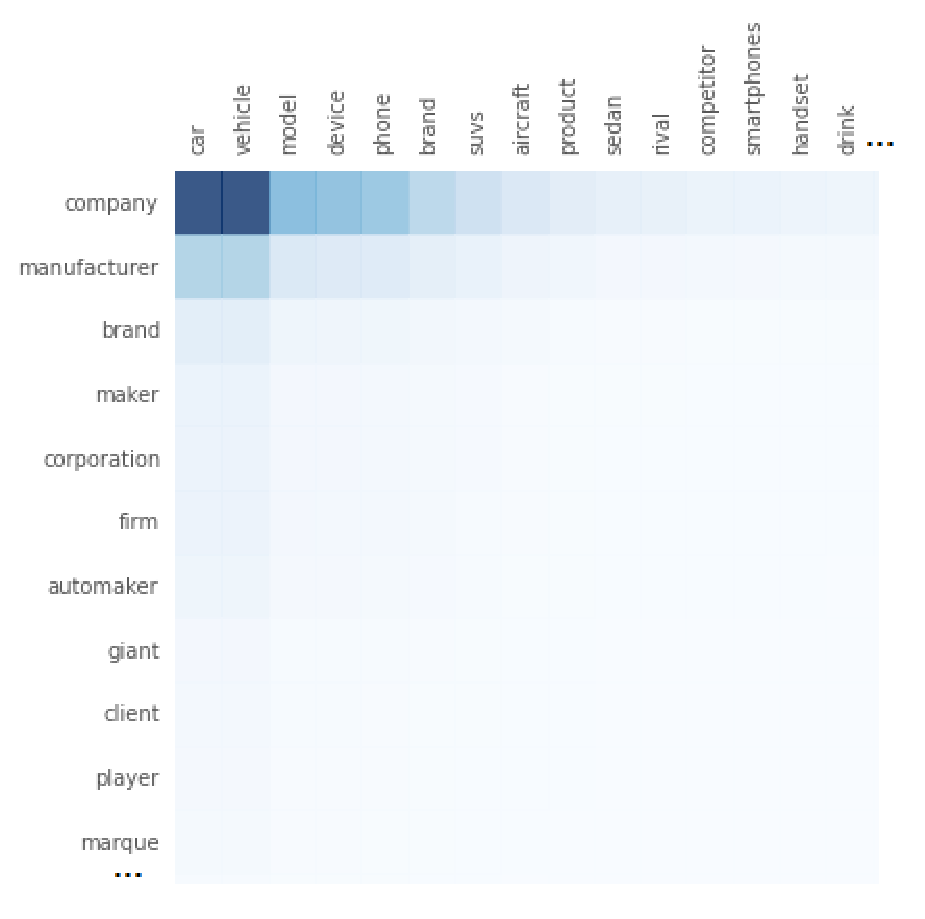
\epsfig{file=resources/ev_plot_manufacturer.eps,width=2.5in}
%\caption{$(c_1,c_2$) plot for attribute \term{Manufacturer}. } \label{fig:evplot}
%\end{figure}
%
%\begin{example}[Sense Disambiguation]
%Consider the following $(e1,a,e2)$ tuple \term{(iphone, manufacturer, apple)}. Suppose it is our query, where \term{apple}'s sense can either be a kind of \term{fruit} or a \term{company}.
%Fig.~\ref{fig:evplot} is a heatmap for all the concepts pairs $(c_1,c_2)$ of attributes \term{manufacturer}. The horizontal axis represents the $e_1$ and the vertical axis stands for $e_2$. The darker the blue is, the higher typicality it will be. In Fig.~\ref{fig:evplot}, We can observe that the top concepts of $e_2$ in the heatmap are \term{company, manufacturer,...} and top 10 pairs also does not include \term{fruit}. The intuition for this is that there exists thousands of $(e1,a,e2)$ tuple such as \term{(BMW\_Z4,manufacturer,BMW),(PlayStation\_4,manufacturer,Sony)} other than \term{(iphone, manufacturer, apple)} tuple, which results in a reasonable distribution.
%\label{exa:sd}
%\end{example}
%
%We further present a comparison of Eq.~\ref{eq:target_expand2_jr} and Eq.~\ref{eq:target_expand2_naive}, where the conceptualization is done with and without multiplying $\alpha(c_1,c_2)$.
%
%\begin{figure}[!htb]
%\centering
%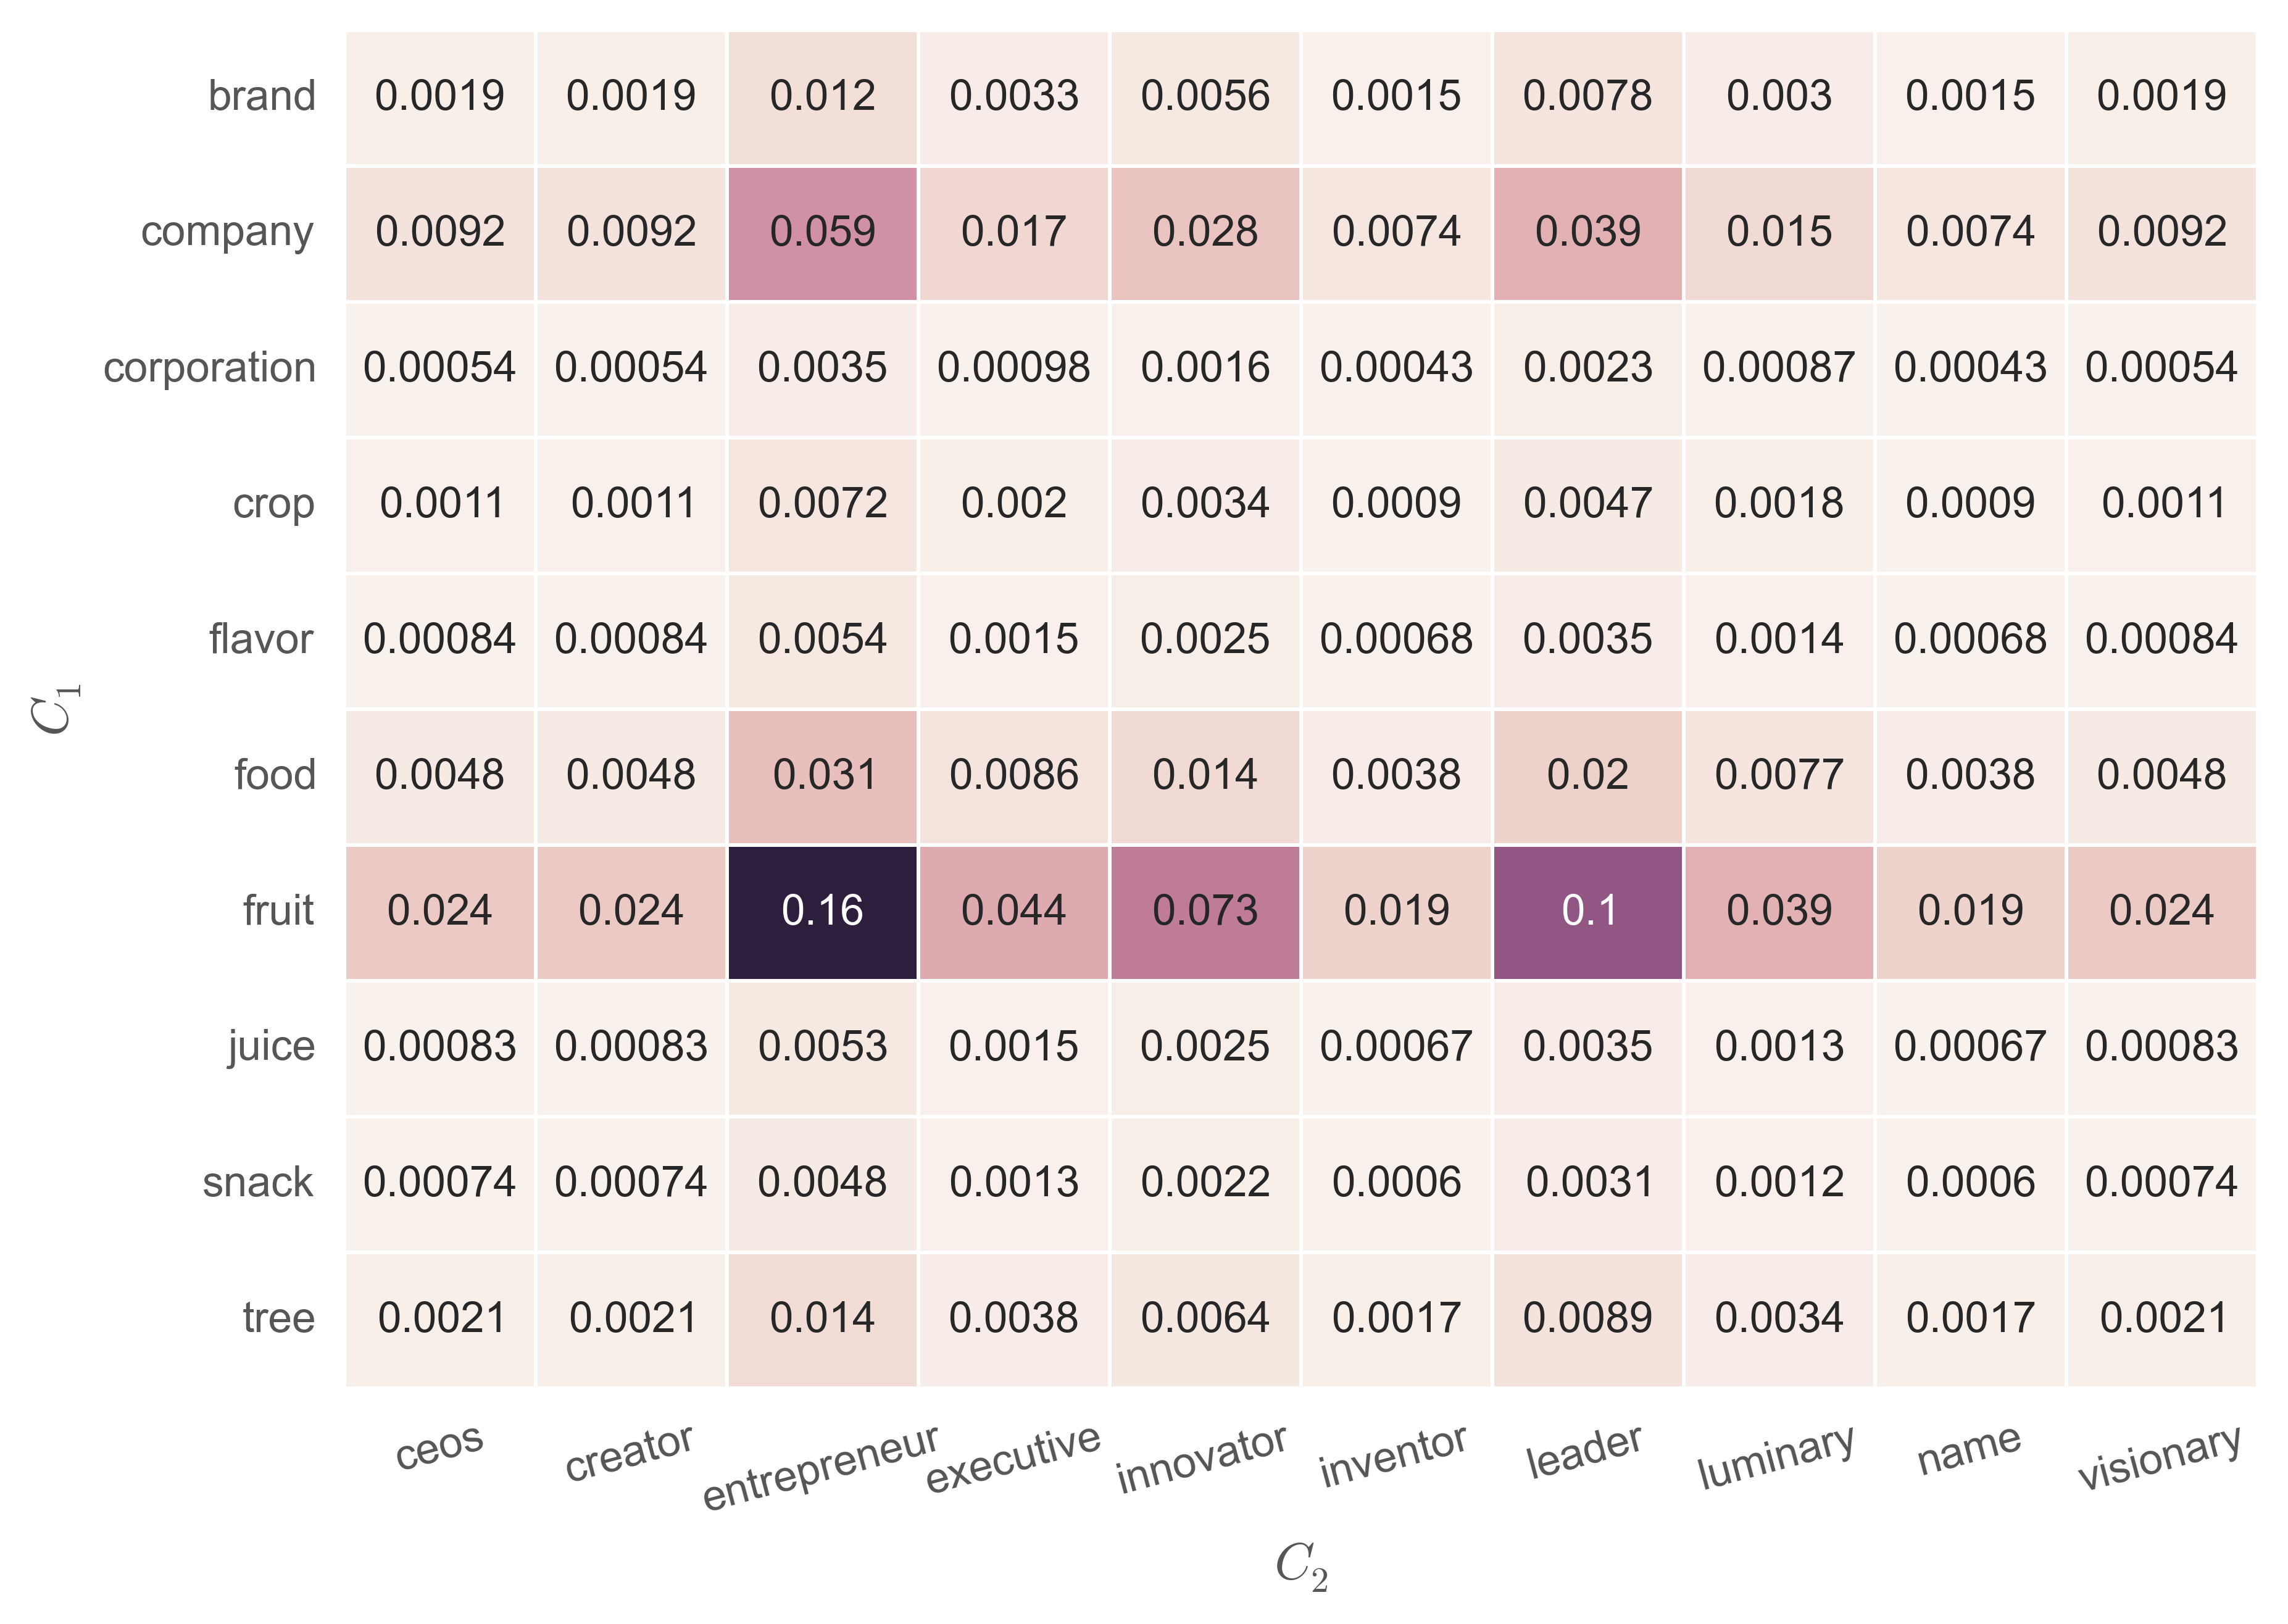
\epsfig{file=resources/df_for_plot_foundedBy.eps,width=\columnwidth }
%\caption{Distribution of $P(\langle c_1,c_2 \rangle|\langle e_1,e_2 \rangle )$ of attribute \at{foundedBy} \textbf{without} $\alpha$. }
%\label{fig:c1c2}
%\end{figure}
%
%\begin{figure}[!htb]
%\centering
%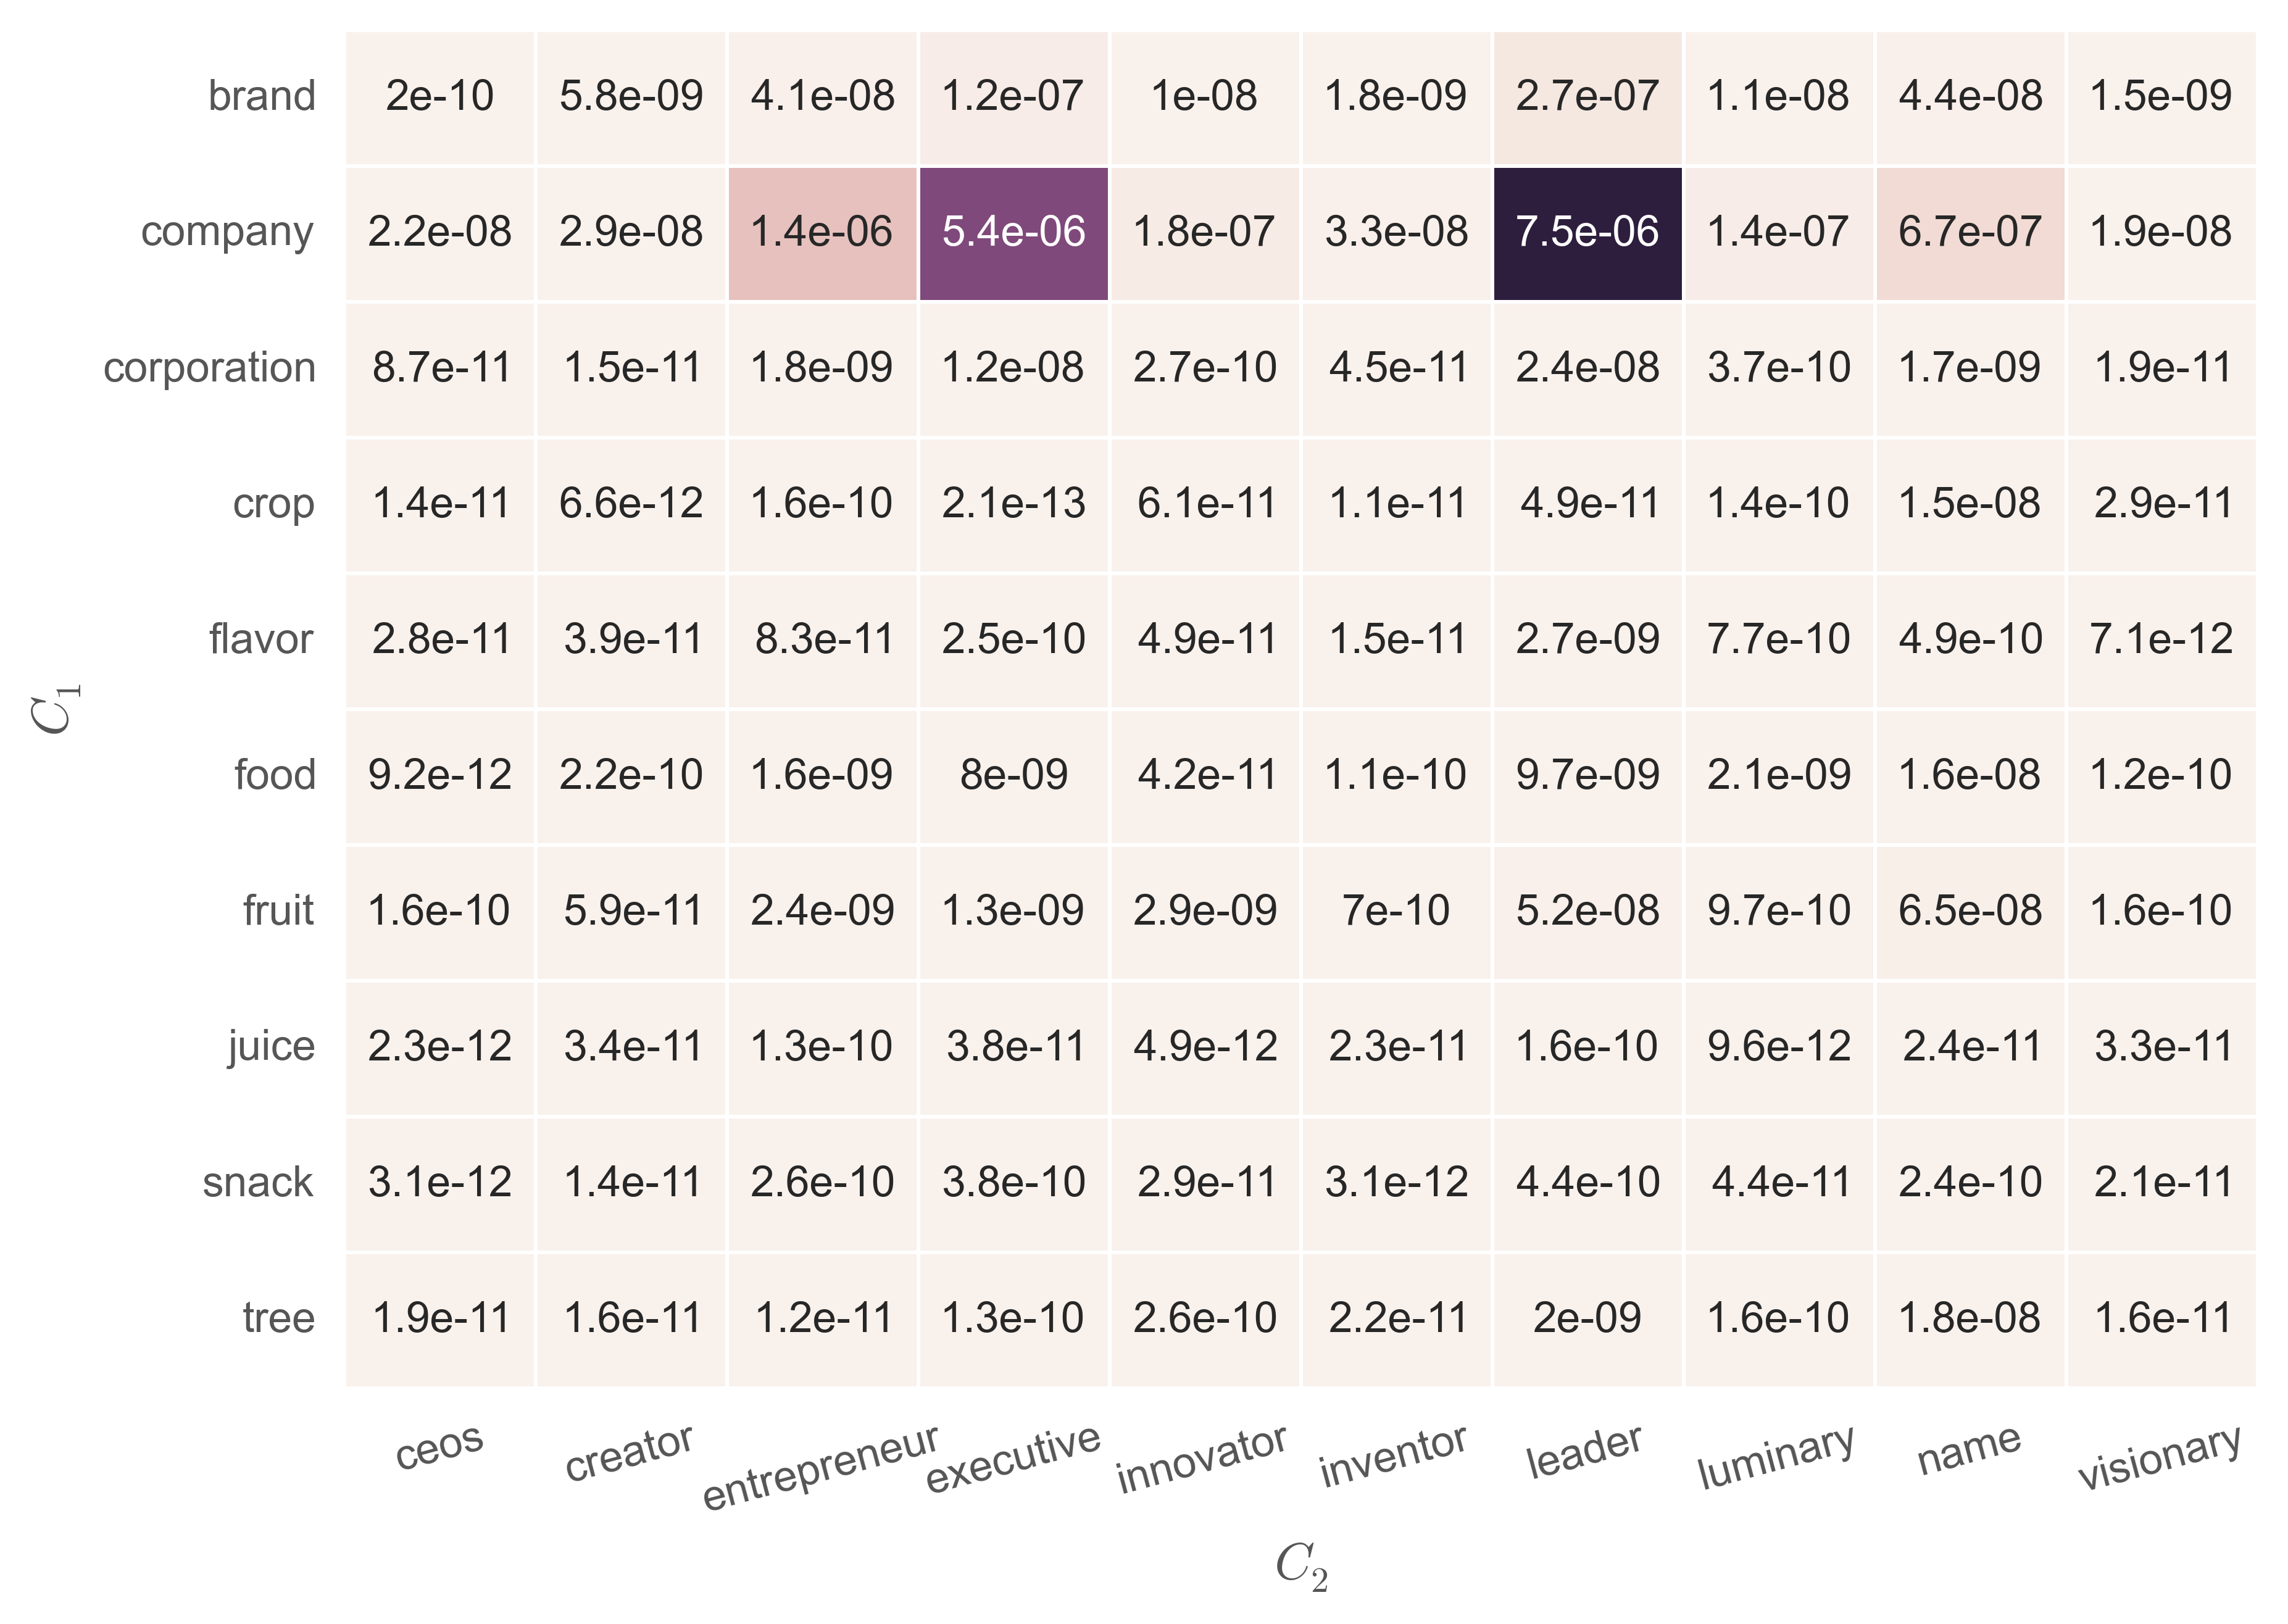
\epsfig{file=resources/df_for_plot_foundedBy_with_alpha_c1c2.eps,width=\columnwidth}
%\caption{Distribution of $P(\langle c_1,c_2 \rangle|\langle e_1,e_2 \rangle )$ of attribute \at{foundedBy} \textbf{with} $\alpha=P(\langle c_1,c_2 \rangle)$. }
%\label{fig:c1c2_alpha}
%\end{figure}
%
%\begin{figure}[!htb]
%\centering
%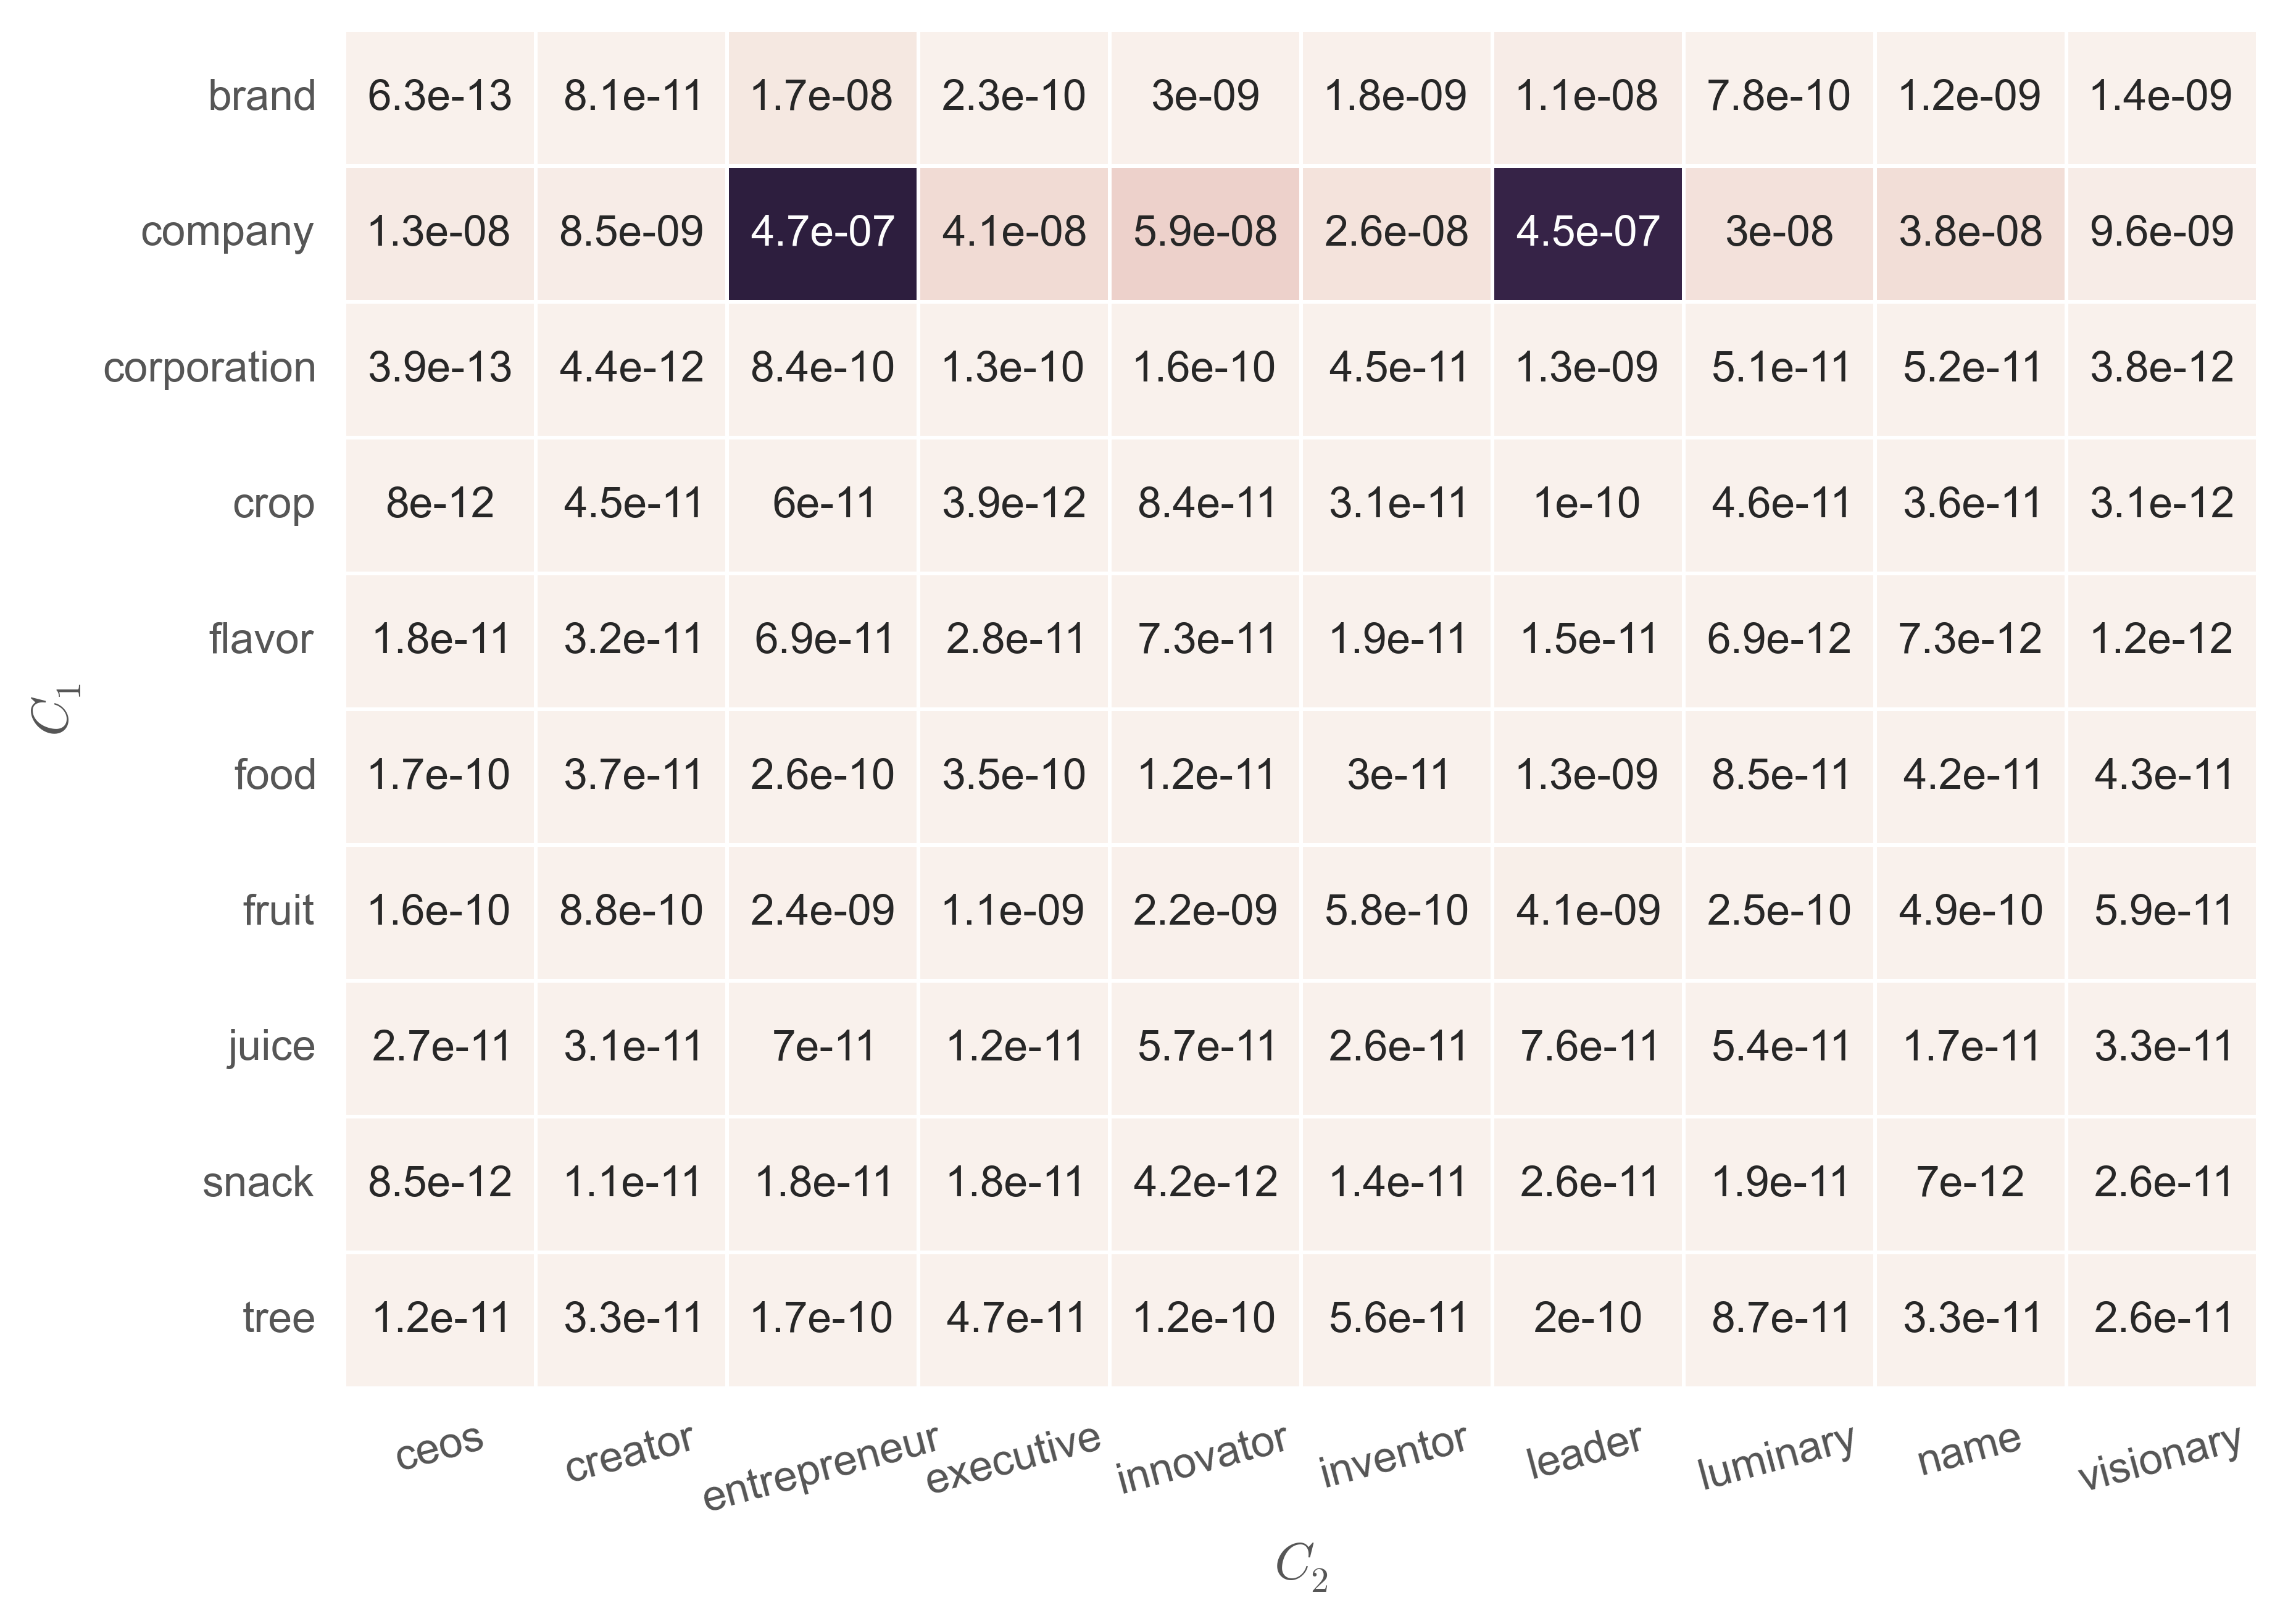
\epsfig{file=resources/df_for_plot_foundedBy_with_alpha.eps,width=\columnwidth}
%\caption{Distribution of $P(\langle c_1,c_2 \rangle|\langle e_1,e_2 \rangle )$ of attribute \at{foundedBy} \textbf{with} $\alpha=P(\langle c_1,c_2 \rangle|a)$. }
%\label{fig:c1c2_alpha_given_a}
%\end{figure}
%
%
%We present the visualization of the distribution of $P(\langle c_1,c_2 \rangle|\langle e_1,e_2 \rangle )$ for Eq.~\ref{eq:naive} in Figure~\ref{fig:c1c2} and for Eq.~\ref{eq:target_expand2_jr} in Figure~\ref{fig:c1c2_alpha}.
%The floats inside each box represents $P(\langle c_1,c_2 \rangle|\langle e_1,e_2 \rangle )$, when the pair $\langle c_1,c_2 \rangle$ does not exist, we add a small value to $\alpha$ and then do normalization for smoothing purpose.

Apparently, the result with $\alpha$ is significantly better. For example it removes the concept level ambiguity of \at{apple} as a \at{fruit}.


\subsection{Exp 4: Collective Conceptulization}
We compare our approach with an $MDL$ based collective conceptualization solution~\cite{sunconceptual}, which aims at generating a minimum set of conceptual labels that best summarize a bag of words.
In our case, the bag of words refers to entities.
$MDL$ use $\alpha$ to tune the balance between \ac{Minimality} and \ac{Coverage}. We set the parameter $\alpha$ in $MDL$ to 0.1 and 0.5 for gaining more results.
We select 50 attributes from different relation groups (such as \ac{PERSON-ORGNIZATION,PERSON-AFFLIATION,OBJECT-LOCATION} etc.\ ) and manually evaluate the top 20 concept pairs in the intersection of results produced by $ERF$ and $MDL$ for each attribute.
We present the human evaluated score in Figure~\ref{fig:eva_violin_pc1c2ga}.

We also show the distribution information on each relation group produced by $ERF$ in Figure~\ref{fig:eva_violin_group}.

\begin{figure}[!htb]
\centering
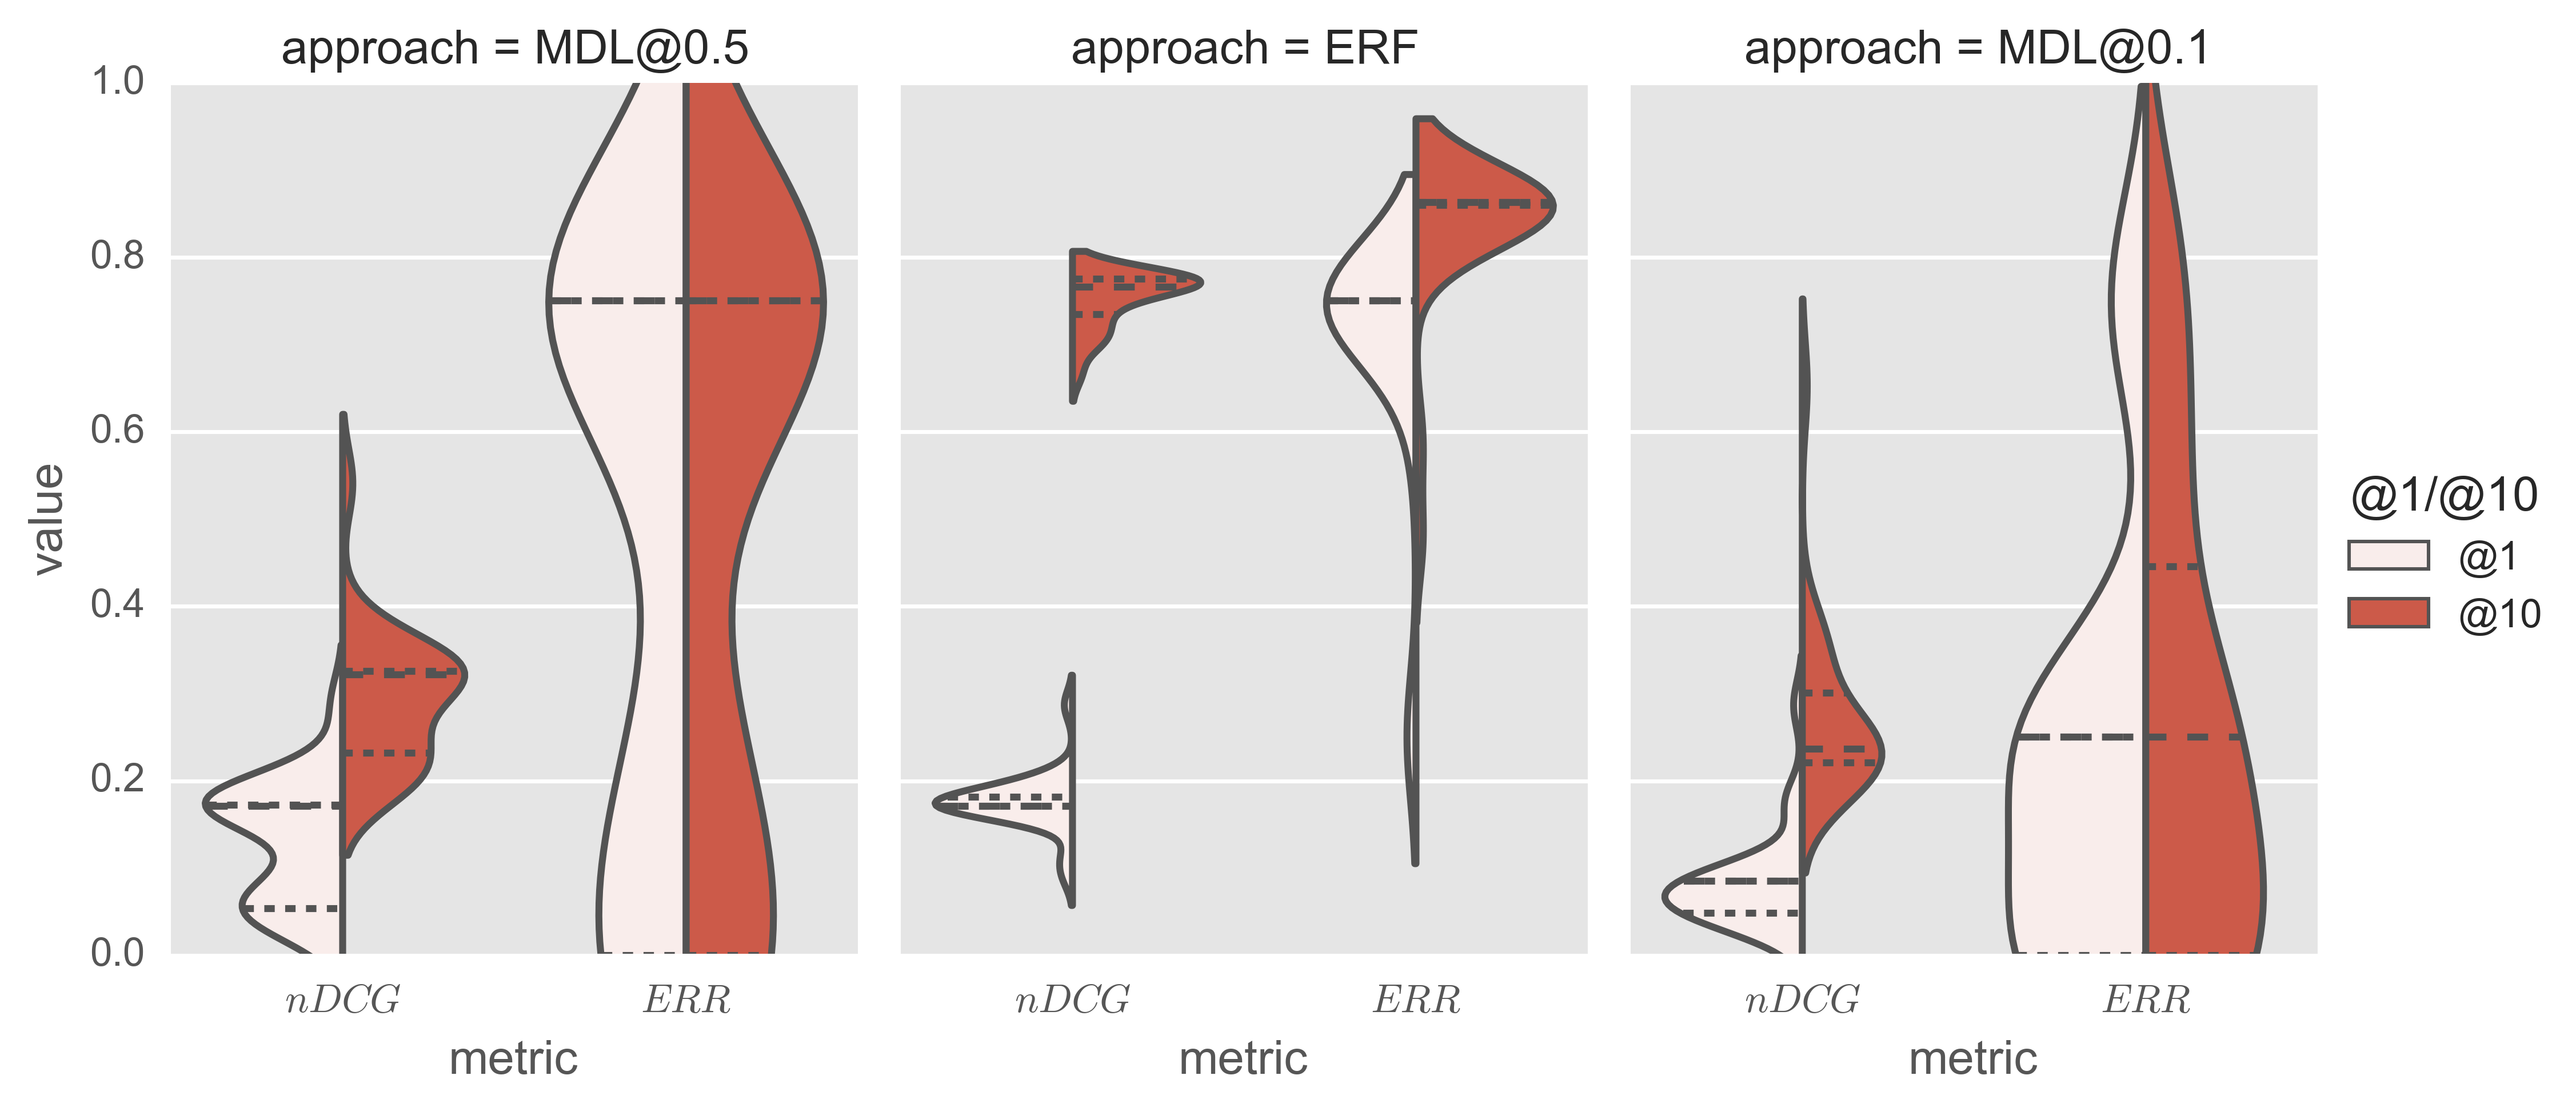
\epsfig{file=resources/violin_eval.eps,width=1.1\columnwidth}
\caption{Distribution of Human Evaluated result for $P(\langle c_1,c_2 \rangle|a)$. \small The white part is metric@1 and the red part is metric@10. Dashed line means quartiles of the distribution. The $ERF$ in the middle is our result, compared with $MDL@\alpha=0.5$(left) and $MDL@\alpha=0.1$(right). }
\label{fig:eva_violin_pc1c2ga}
\end{figure}

The $nDCG@1$ score is reasonably low since the correct concept pair is often more than 1.
We can observe a significant increase in the $nDCG@10$ score in our approach while not much increase in $MDL$-based approach since $MDL$ tends to give as few concepts as possible and sacrifices the coverage when $\alpha$ is small.
The $ERR@1$ and $ERR@10$ mesure varies not that much due to its user behavioral instinct of not searching forward when find the concept.
The $ERF$ provides rich correct concept pairs to handle the long-tailed concept pairs and gain an slight increase in $ERR@10$

\begin{figure*}[!htb]
\centering
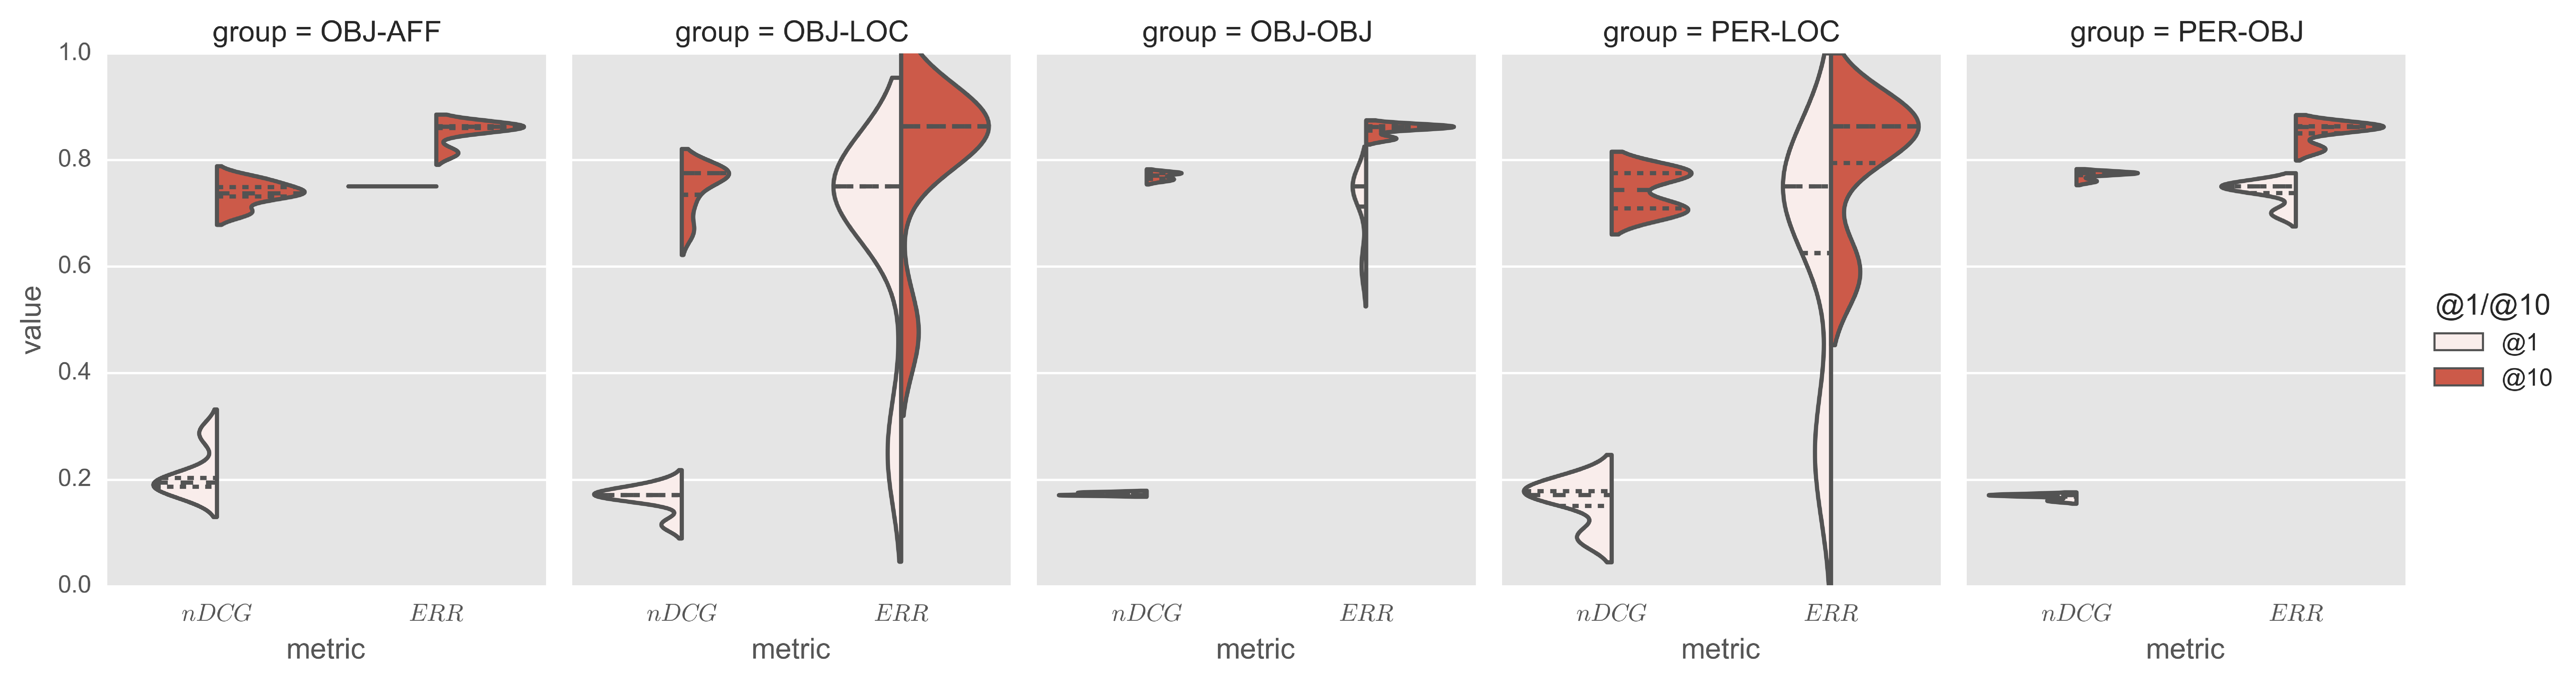
\epsfig{file=resources/violin_eval_group.eps,width=2.2\columnwidth}
\caption{Distribution of Human Evaluated result for $P(\langle c_1,c_2 \rangle|a)$ produced by $ERF$. \small Each seperate graph represents a relations group.}
\label{fig:eva_violin_group}
\end{figure*}



\subsection{Case Study}

We show some of the relations that has been retrieved by our method in Table~\ref{tab:results}.
The first 2 columns show the query entity pair.
The 3rd column is the relation retrieved by ERF with a confidence score in the 4th column.
Note that we combine the relation of $\langle e_1,e_2\rangle$ and $\langle e_2,e_1\rangle$ into one single result.
For example the relation \at{commander} of \at{<adolf hitler,world war ii>} is actually that of \at{<world war ii, adolf hilter>}
% Table generated by Excel2LaTeX from sheet 'Sheet1'
\begin{table}[ht!]
  \centering
  \caption{First three results produced by ERF}
    \begin{tabular}{cccr}
    \toprule
    Entity1 & Entity2 & Relation & Score \\
    \midrule
    \multicolumn{1}{c}{\multirow{3}{*}{\parbox{1cm}{ Sherlock Holmes}}} & \multicolumn{1}{c}{\multirow{3}[0]{*}{united kingdom}} & anthem & 0.007079 \\
    \multicolumn{1}{c}{} & \multicolumn{1}{c}{} & firstAppearance & 0.004487 \\
    \multicolumn{1}{c}{} & \multicolumn{1}{c}{} & allegiance & 0.004357 \\
    \hline
    \multicolumn{1}{c}{\multirow{3}{*}{\parbox{1cm}{\centering apple}}} & \multicolumn{1}{c}{\multirow{3}[0]{*}{steve jobs}} & foundedBy & 0.015439 \\
    \multicolumn{1}{c}{} & \multicolumn{1}{c}{} & keyPerson & 0.009932 \\
    \multicolumn{1}{c}{} & \multicolumn{1}{c}{} & successor & 0.008069 \\
    \hline
    \multicolumn{1}{c}{\multirow{3}{*}{\parbox{1cm}{\centering Adolf Hitler}}} & \multicolumn{1}{c}{\multirow{3}[0]{*}{world war ii}} & commander & 0.037712 \\
    \multicolumn{1}{c}{} & \multicolumn{1}{c}{} & battle & 0.022161 \\
    \multicolumn{1}{c}{} & \multicolumn{1}{c}{} & ceo   & 2.44E-05 \\
    \hline
    \multicolumn{1}{c}{\multirow{3}{*}{\parbox{1cm}{\centering Microsoft}}} & \multicolumn{1}{c}{\multirow{3}[0]{*}{redmond}} & locationCity & 0.082507 \\
    \multicolumn{1}{c}{} & \multicolumn{1}{c}{} & foundationPlace & 0.047192 \\
    \multicolumn{1}{c}{} & \multicolumn{1}{c}{} & location & 0.036916 \\
    \hline
    \multicolumn{1}{c}{\multirow{3}{*}{Titanic}} & \multicolumn{1}{c}{\multirow{3}[0]{*}{James Cameron}} & director & 0.124407 \\
    \multicolumn{1}{c}{} & \multicolumn{1}{c}{} & cinematography & 0.096447 \\
    \multicolumn{1}{c}{} & \multicolumn{1}{c}{} & editing & 0.080134 \\
    \hline
    \multicolumn{1}{c}{\multirow{3}{*}{Titanic}} & \multicolumn{1}{c}{\multirow{3}[0]{*}{Leonardo Dicaprio}} & starring & 0.049689 \\
    \multicolumn{1}{c}{} & \multicolumn{1}{c}{} & narrator & 0.037267 \\
    \multicolumn{1}{c}{} & \multicolumn{1}{c}{} & producer & 0.01306 \\
    \hline
    \multicolumn{1}{c}{\multirow{3}{*}{\parbox{1cm}{\centering Harry Potter}}} & \multicolumn{1}{c}{\multirow{3}[0]{*}{J K rowling}} & notableWork & 0.016965 \\
    \multicolumn{1}{c}{} & \multicolumn{1}{c}{} & author & 0.015514 \\
    \multicolumn{1}{c}{} & \multicolumn{1}{c}{} & coverArtist & 0.014906 \\
    \bottomrule
    \end{tabular}%
  \label{tab:results}%
\end{table}%


%\subsection{Selectional Preference}
